\documentclass{article}
\usepackage{titling}
\usepackage{lipsum}
\usepackage{amsmath}
\usepackage{listings}
\usepackage{graphicx}
\usepackage{subcaption}
\usepackage{pgfplots}
\usepgfplotslibrary{statistics}



\begin{document}
\noindent
\begin{minipage}[t]{0.6\textwidth}
    \begin{flushleft}
        \LARGE\textbf{Math 343 - Lab 3} \\
        \vspace{6pt} % add 6pt of vertical space
        \hrule width 10cm
        \vspace{12pt}
        \large\textbf{Preston Duffield} \\
        \large Western Washington University \\
        % \today
        April 18, 2023
        \vspace{24pt}
    \end{flushleft}
\end{minipage}

\section*{a)}
The hypothesis for the test is: \\
$H_0$: $\mu_1 = \mu_2 = \mu_3$. \\
$H_a$: At least one $\mu_i$ is different. \\
The test statistic $F = 7.91$. \\
The P-value = 0.006. \\
Since the P-value$< \alpha = 0.5$ we can conclude the following:
There is not enough statistic evidence to support the hypothesis that $\mu_1 = \mu_2 = \mu_3$.

\section*{b)}
An estimate of the overall mean $\mu$, is given by the following:
\begin{align*}
    \hat{\mu} &= \frac{1}{a} \sum_{i=1}^{a} \hat{\mu_i} \\
              &= (13.4 + 38.2 + 73) / 4 \\
              &= 41.5\bar{3} \\
\end{align*}
An estimate of the variance $\sigma^2$ of the random error term $\epsilon_{ij}$ can be pulled from the pooled standard deviation in Minitab:
\begin{align*}
    S_p ^2 &= 23.7978^2 = 566.335
\end{align*}

\clearpage
\section*{c)}
\begin{figure}[h]
    \centering
    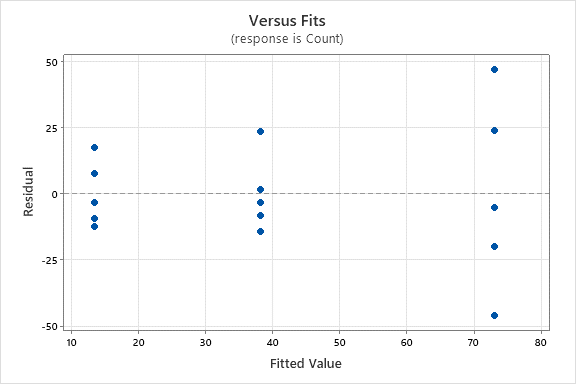
\includegraphics[width=1\textwidth]{./images/c.png}
    \caption{The residual plot from Minitab.}
    \label{fig:c}
  \end{figure}
The residual plot seems to indicate heteroskedasticity. The data appears to have a bell like shape where data with a lower fitted value has a smaller residual spread.
\section*{d)}
\section*{e)}
\section*{f)}
\section*{g)}
\section*{h)}


\end{document}